% !TeX root = ../main.tex

\chapter{多二值特征图方法设计}

\section{概述}

近年来,二值神经网络因极低的资源消耗受到人们的关注,但是二值神经网络的精度与同结构浮点网络相比仍有较大差距。二值网络较弱的模型能力是其性能较差的主要原因之一。权重的二值化和激活值的二值化导致了网络模型函数拟合能力和特征表达能力弱化,研究人员提出了很多方法解决这两个二值化过程的信息损失问题。对于权重二值化,权重是神经网络的可学习参数,神经网络训练的目的就是优化权重,因此可以从优化角度对权重进行调整,例如设计二值权重友好的损失函数项。权重参数在推理过程中不变,没有必要在网络训练完成后保留二值权重的浮点前身,因此可以设计复杂的权重二值化函数来提升二值权重的优化能力\cite{xu2021layerwisea}。上述方法都可以增强权重在反向传播中的优化能力,使二值神经网络在有限的函数空间中尽可能逼近真实任务函数。对于激活值二值化,则无法使用权重二值化的设计思路。激活值在网络中的作用导致其二值化有两个限制条件。一是动态性要求,激活值是神经网络的中间结果,由神经网络的前向传播过程中动态计算而来,网络输入变化激活值也会随之改变。激活值不是神经网络训练时的最终优化对象,因此无法在训练时使用额外的损失函数项约束激活值的二值化过程。二是复杂性要求,激活值的二值化过程不能过于复杂。由于在推理时网络可以只存储二值权重,因此可以为权重设计复杂的二值化过程。但是激活值是在推理时动态计算生成的,神经网络二值化的目的是减少网络推理的资源消耗,复杂的二值化过程可能抵消二值卷积的低计算量优势,使二值网络的设计失去意义。

激活值二值化过程是二值神经网络必须具备的环节,也是二值神经网络性能的瓶颈。本文提出了多二值特征图方法,该方法突破了一张浮点特征图二值化为一张二值特征图的限制,将一张浮点特征图使用不同的二值函数转换为不同的二值特征图,多个二值特征图从不同的角度保留原浮点特征图的信息,从而减少激活值二值化过程中的信息损失,提升网络性能。考虑到激活值二值化的两个限制条件,多二值特征图方法使用不同阈值的符号函数作为不同的二值函数,符号函数的简洁性使激活值二值化过程只增加了一个逐元素加法运算。多二值特征图方法的重点是如何选择选择对同一浮点特征图进行处理的不同的二值函数,具体来说是符号函数的不同阈值。本文提出二值特征相似度来衡量从一张浮点特征图得到的多张二值特征图时保留信息的能力,并以此为标准设计最优的多二值特征图个数和合适的阈值取值。手工搜索选取的阈值可以实现较好的效果,本文更进一步研究了多个阈值的自动选取方法,设计了大量的实验尝试阈值的选择。通过对实验结果的分析得到,阈值参数既不适合动态计算得到,也不适合当作普通参数与权重一起训练,而是应被当作二值神经网络的结构参数。本文提出使用双层规划的方法对阈值进行自动优化,实现了阈值的自动选取,并通过实验验证了自动选取的阈值可以达到手工设计的阈值的效果。

\section{多二值特征图算法}

增加网络宽度是提升二值网络特征表示能力的主要手段之一。MeliusNet\cite{meliusnet}通过增加网络每层特征的通道数增强了模型能力,该方法对卷积的输入和输出通道数都进行了扩增。在二值网络的一个卷积块中,卷积层的输入是二元值,输出是整数值,卷积输出经过归一化层和激活层后转变为实数值,该实数值传递给下一个卷积块时会经过二值函数转换为二元值。可以看到,信息的损失发生在二值函数处,即浮点特征向二值特征的转化中,增加特征通道数虽然从整体上提升了网络能力,但是二值化过程仍然是一张浮点特征图得到一张二值特征图的一对一的转换,仍然造成从32位到1位的信息损失,没有高效地利用网络增加的宽度。ABC-Net\cite{abcnet}将一个浮点激活值用多个二值激活值组合表示,相当于增加了网络的宽度,但是其思路是减小量化误差,即多个二值激活值的加权和尽可能接近原浮点激活值。该方法中多个二值激活值共用一组权重,限制了权重对不同二值特征图的解析能力。本文提出的多二值特征图方法弥补了上述方法的缺点。与MeliusNet相比,本文方法可以更高效的利用通道数,对于扩增$n$张二值特征图的情况,本文方法实现了从32位到$n$位的信息损失。与ABC-Net相比,本文方法每张二值特征图都使用独立的权重进行解析,从而使网络获得更好的特征解析能力。

\subsection{特征扩增方法}

本文提出的多二值特征图方法使用不同的二值函数将同一张浮点特征图转换为不同的二值特征图,定义不同二值特征图的个数为扩增倍数$n$。图 \ref{fig:multifeature} 展示了浮点特征图通道数为3,扩增倍数$n = 3$时的多二值特征图方法,其中$\phi_1$、$\phi_2$、$\phi_3$分别表示3个不同的二值函数,经过扩增后二值特征图的总通道数为9,每3个通道对应1张浮点特征图,也就是1张浮点特征图的信息由3张二值特征图保留,不同二值函数的特征扩增后,所有二值特征图都会作为后续卷积的输入,经过神经网络普遍的处理流程后,将再次得到3张浮点特征图。值得注意的是本方法虽然扩增了卷积输入的通道数,但是保持了卷积输出的通道数不变。因此与单纯增强通道数相比,本方法在相同的二值特征图数量的条件下减少了$n$倍的计算量。本方法中扩增得到的二值特征图都作为独立的通道参与后续的卷积运算,因此每张二值特征图都会学习独立的权重卷积核,这可以最大化利用神经网络训练的自适应性,为每个通道的二值特征寻找权重参数。

\begin{figure}[htb]
  \vspace{6pt}
  \centering
  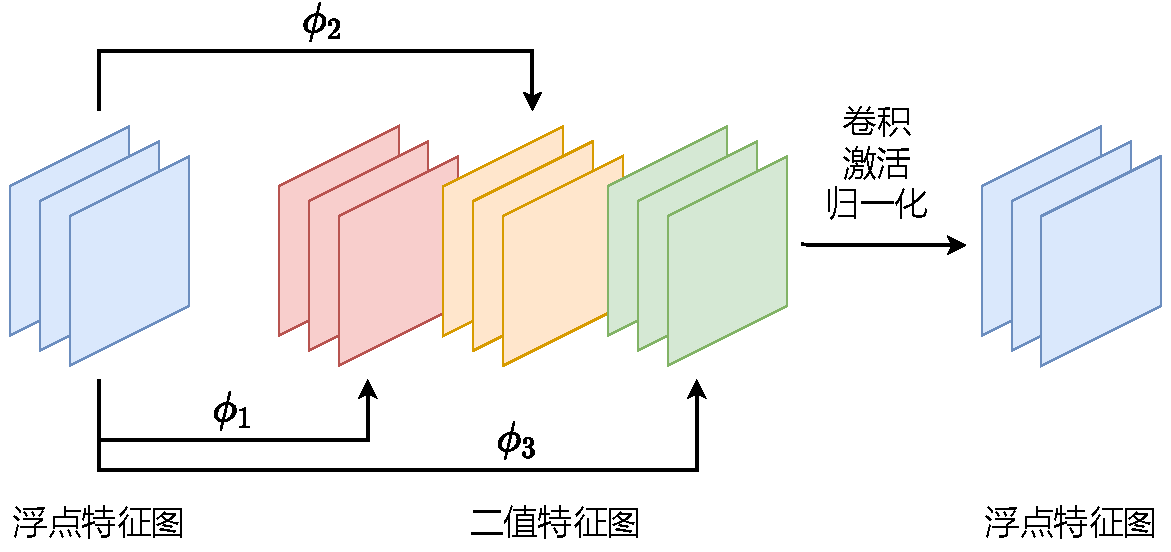
\includegraphics[width=0.95\textwidth]{multifeature.pdf}
  \caption{多二值特征图方法示意图}
  \label{fig:multifeature}
\end{figure}

\subsection{二值函数}

多二值特征图方法的核心是不同的二值函数,本文使用阈值可变的符号函数作为二值函数,定义为公式 \eqref{eq:sign_a}:

\begin{equation}
  \label{eq:sign_a}
  sign_\alpha(x) =
  \begin{cases}
    -1 & if \ x < \alpha \\
    +1 & if \ x \geq \alpha 
  \end{cases},
\end{equation}
其中$x$表示激活值,$\alpha$表示符号函数的阈值,$sign_\alpha$表示阈值可变的符号函数,该函数逐元素的作用在浮点特征图的每一个激活值上,一一对应的得到二值特征图的每一个元素。可变阈值的符号函数实现十分简单,充分符合激活值的二值函数的复杂性要求。在实际应用中,可以用先对浮点特征图进行$\alpha$的整体偏移,然后应用阈值为0的普通符号函数的方法代替可变阈值符号函数,每个二值函数只需执行一次逐元素加法和取符号运算即可。

神经网络使用梯度下降法进行训练,激活值的二值化过程作为网络中间过程必须能够计算梯度,但符号函数阈值处无导数,阈值外区域导数为0,无法进行梯度计算。参考Bi-real Net\cite{birealnet},在反向传播时本文使用多项式近似的截断函数代替阈值可变符号函数,定义为公式 \eqref{eq:psign}:

\begin{equation}
  \label{eq:psign}
  psign_\alpha(x) = 
  \begin{cases}
    -1 & if \ x < \alpha - 1 \\
    2(x - \alpha) + (x - \alpha)^2 & if \ \alpha - 1 \leq x < \alpha \\
    2(x - \alpha) - (x - \alpha)^2 & if \ \alpha \leq x < \alpha + 1 \\
    +1 & if \ x \geq  \alpha + 1
  \end{cases},
\end{equation}
其中$psign_\alpha$表示符号函数的多项式近似函数,该函数将激活值截断到$(-1, 1)$的范围内,自变量$x \in (\alpha - 1, \alpha + 1)$时为分段的二次多项式函数,该函数的梯度函数为公式 \eqref{eq:psign_d}:

\begin{equation}
  \label{eq:psign_d}
  \frac{\partial psign_\alpha(x)}{\partial x} = 
  \begin{cases}
    2 + 2(x - \alpha) & if \ \alpha - 1 \leq x < \alpha \\
    2 - 2(x - \alpha) & if \ \alpha \leq x < \alpha + 1 \\
    0 & \text{otherwise}
  \end{cases},
\end{equation}
可以看到,自变量$x \in (\alpha - 1, \alpha + 1)$时该近似函数梯度不为0,可以正常进行梯度反向传播,其他情况下梯度为0。这样做可以限制激活值的取值范围,当激活值取值过大时就不会进行更新,减少激活值的二值量化误差。

不同阈值的符号函数可保留浮点特征图中的不同信息,如图 \ref{fig:different_thres} 所示,第一行是浮点特征图,第二行是分别使用阈值为0.6、0、-0.6的符号函数得到的二值特征图。可以看到符号函数将特征划分成了两个部分,不同阈值得到的二值特征图会突出不同的特征,即从不同的角度保留信息,较大的阈值重点提取浮点特征中数值较大的部分,而平滑掉其他部分,较小的阈值正好相反。通过合理地选择阈值,可以减少多张二值特征图保留的信息的重复,增加二值特征的利用率。

\begin{figure}[htb]
  \vspace{6pt}
  \centering
  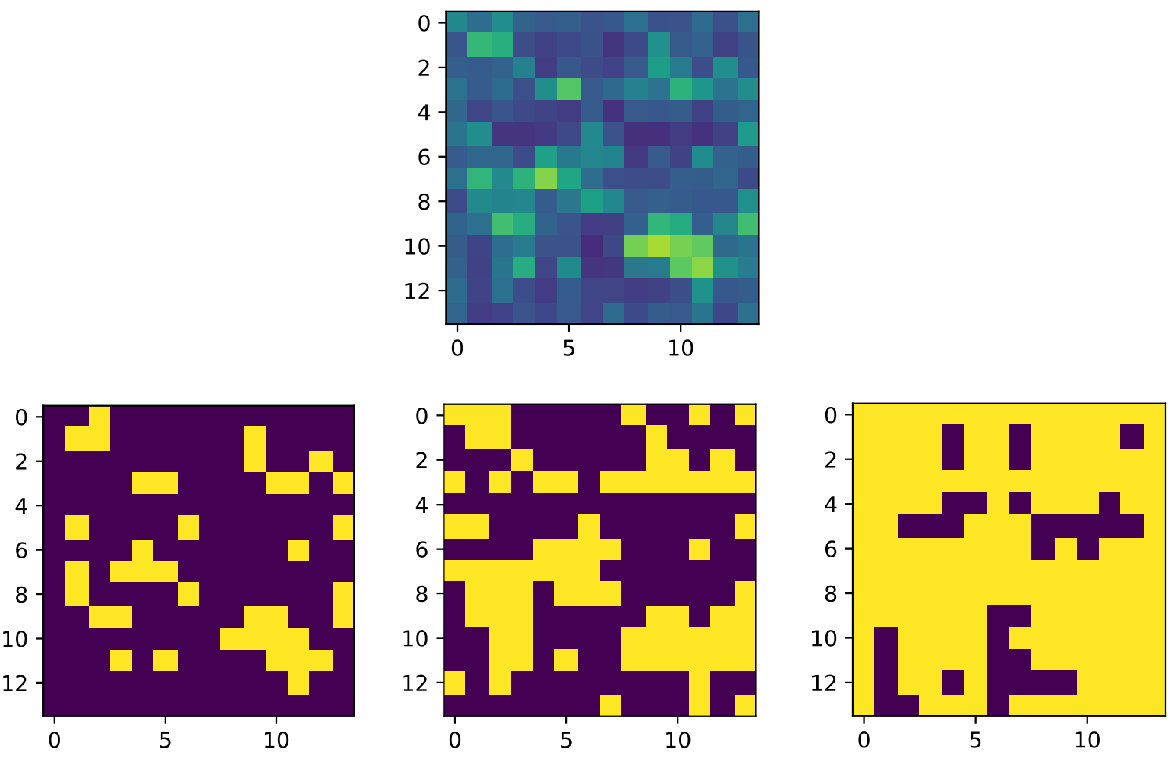
\includegraphics[width=0.75\textwidth]{different_thres.pdf}
  \caption{不同阈值符号函数得到二值特征图示意图}
  \label{fig:different_thres}
\end{figure}

\section{多特征图信息保留能力评价指标}

为了能够指导阈值的设置策略,本文对衡量不同二值特征图的信息保留能力的方法进行了研究。二值特征图每个元素的取值$x \in \{-1, +1\}$,总元素个数为$N$的二值特征图所能表示的不同特征为$2^N$个。由于总元素个数为$N$的浮点特征图能表示的不同特征有$32^N$个,因此二值特征图的特征空间远小于浮点特征图,二值特征图只能从浮点特征图中保留极其有限的信息。在多二值特征图方法中,我们使用多个不同的二值函数从同一浮点特征图提取不同的二值特征,扩增倍数为$n$时,多张二值特征图联合的特征空间有$n \cdot 2^N$种取值。理论上不同二值特征保留的信息差异越大,扩增后的特征空间的利用率就越高,多二值特征图方法的性能越好,因此需要对不同二值特征图保留信息的差异性进行定量的分析。

\subsection{二值特征相似度}

有很多研究从量化误差的角度分析二值化前后特征的信息保留效率,但是目前为止没有人研究过从同一浮点特征提取到的不同二值特征的差异性。本文首次提出使用二值特征相似度作为衡量两个二值特征差异性的评价指标,二值特征相似度定义如公式 \eqref{eq:bfs} 所示:

\begin{equation}
  \label{eq:bfs}
  BFS(\bm{x}_1, \bm{x}_2) = \frac{|\bm{x}_1 \cdot \bm{x}_2|}{||\bm{x}_1||\cdot||\bm{x}_2||},
\end{equation}
其中$\bm{x}_1$和$\bm{x}_2$表示两个二值特征向量,函数$BFS(\cdot, \cdot)$表示两个二值特征向量计算得到的二值特征相似度,当计算两张二值特征图的二值特征相似度时,需要以相同的方式将两张二值特征图转换为一维的二值特征向量进行计算。可以发现,二值特征相似度本质上是向量的余弦相似度取绝对值得到的。余弦相似度计算的是两个向量的夹角,可以从整体上衡量两个向量的差异,这与神经网络中的特征十分契合,神经网络的特征在计算过程中表现为特征图,单看一个元素没有意义,元素间的相对大小关系才承载着特征图中真正的信息。对余弦相似度取绝对值是二值特征独有的特点,在二值特征图中,两个元素取值要么相等,要么互为相反数,因此两个二值特征余弦夹角大小相等,符号相反时承载了相同的信息。例如一张全$+1$的二值特征图和一张全$-1$的二值特征图本质上包含了相同的信息,在神经网络推理时,只需要将权重全部取相反数,这两张二值特征图就可以得到完全相同的推理结果,在神经网络训练时,对特征图乘以$-1$对训练结果没有任何影响,这是由于权重学习的自适应性,可以将特征图上乘的$-1$吸纳到权重参数中。

对于从同一浮点特征提取的多个二值特征,本文使用所有二值特征两两之间的二值特征相似度的均值作为总二值特征相似度,如公式 \eqref{eq:bfs_all} 所示:

\begin{equation}
  \label{eq:bfs_all}
  BFS(\bm{x}_1, \bm{x}_2, \dots, \bm{x}_n) = \frac{2}{n(n-1)} \sum_{i = 1}^{n} \sum_{j = i+1}^{n} BFS(\bm{x}_i, \bm{x}_j),
\end{equation}
其中$n$表示二值特征的个数,$\bm{x}_1, \bm{x}_2, \dots, \bm{x}_n$分别表示$n$个二值特征。总二值特征相似度越小,表明多个二值特征之间的差异越大,特征扩增的利用率越高。

经过实验验证,本文提出的二值特征相似度评价指标可以有效衡量从同一浮点特征提取到的多个二值特征的相似性,在相同扩增倍数下,网络的二值特征相似度越小,网络的推理精度越高,具体的实验分析将在3.5节详细介绍。

\subsection{基于二值特征相似度的损失函数项}

由于二值特征相似度可以衡量多特征图方法的有效性,因此也可以指导网络的训练过程。本文提出将网络中所有多特征图方法得到的二值特征图的二值特征相似度作为神经网络训练优化目标的一部分,指导权重参数的学习。基于二值特征相似度的损失函数项如公式 \eqref{eq:loss_sim} 所示:

\begin{equation}
  \label{eq:loss_sim}
  L_{sim} = \sum_{i = 1}^{M} \sum_{j = 1}^{C_i} BFS(\bm{x}_1^{i, j}, \bm{x}_2^{i, j}, \dots, \bm{x}_n^{i, j}),
\end{equation}
其中$M$是神经网络卷积层的总层数,$C_i$表示第$i$层卷积的通道数,$\bm{x}_n^{i, j}$表示第$i$层卷积第$j$个通道的浮点特征图扩展出的第$n$张二值特征图,可以看到,该损失函数项是将网络中所有计算得到的二值特征相似度累加在一起得到的。包含二值特征相似度损失函数项的网络总损失函数可以表示为公式 \eqref{eq:loss}:

\begin{equation}
  \label{eq:loss}
  L = L_{ce} + \theta L_{sim},
\end{equation}
其中$L$为网络总损失函数,$L_{ce}$是用于图像分类任务的交叉熵损失函数项,$L_{sim}$是二值特征相似度损失函数项,$\theta$是$L_{sim}$的加权系数,用于调整这两个损失函数项的比例,该参数需要根据具体的网络架构针对性设定。

当多个二值函数的阈值固定时,使用基于二值特征相似度的损失函数项可以从权重角度继续发掘多特征图方法的潜力,从而保留更多的浮点特征信息,3.5节的实验表明该损失函数项可以一定程度的提高网络的性能。

\section{多特征图阈值设置策略}

\subsection{二值网络阈值参数分析}

二值神经网络前向传播时普遍使用符号函数作为二值函数,符号函数的阈值的设置会对网络的性能产生很大的影响。Kim等人研究\cite{unbalance}表明仅仅通过改变二值神经网络中符号函数阈值的取值,就可以使网络在ImageNet数据集上推理Top1精度提高$0.5\% \sim 3.0\%$。但是如何设置阈值是二值神经网络中的难题,ReActNet\cite{reactnet}使用RSign符号函数自适应地学习阈值参数,该方法将阈值参数作为网络参数的一部分进行优化,优化方法和权重参数相同,本文通过复现消融实验表明这种优化方法无法有效优化阈值参数,使用该方法优化阈值参数的网络精度与直接固定阈值训练的网络精度相差无几。Kim等人\cite{unbalance}同样研究了阈值参数的可学习性,并表明阈值参数是否可以自动学习与网络结构有密切相关,当二值化符号函数和归一化层相连时,阈值参数会融入归一化层参数,失去作为阈值参数的意义。

本文的多二值特征图方法使用不同阈值的符号函数作为不同二值函数,无法使用默认的阈值为0的符号函数,因此本文尝试了多种设置阈值的方法:

\begin{itemize}
  \item 手工设置阈值:根据浮点网络特征图的分布手工设置几个阈值的值,并在二值网络训练中始终保持不变;
  \item 输入自适应阈值:根据网络前向传递时浮点特征图的数值信息动态计算阈值,例如以均匀划分浮点特征图元素的取值范围、均匀划分浮点特征图元素个数等;
  \item 可学习阈值:将阈值作为可学习参数,跟随网络权重一同训练。
\end{itemize}
实验表明,在相同网络结构和训练配置下,使用手工设置的固定阈值方法训练的网络精度最高。

结合他人研究成果和本文实验,本文提出二值网络阈值参数应当作为结构性参数看待,即二值网络阈值参数是网络结构的一部分。结构参数概念首次出现在神经网络结构搜索方法\cite{zoph2017neural}中,其中结构参数用于配置不同的网络结构,网络原有的权重参数被称为非结构参数。结构参数与非结构参数无法同时训练,在二值神经网络中,训练过程中阈值的不断变化相当于网络结构在不断变化,每层网络提取特征的方式也随之变化,使得之前学习到的权重参数不适应新的特征提取方法,拖累了权重的学习。这解释了手工设置固定阈值优于可学习阈值的原因,固定阈值的二值网络结构在训练中不变,优化器可以专注于针对该结构优化权重,可学习阈值在训练中不断变化,使权重优化方向不专一,从而减慢了权重的优化,因此在相同的训练代数下结果差于固定阈值,3.5节的实验验证了这一观点。

\subsection{多特征图阈值自适应优化方法}

本文认为二值网络阈值是结构参数,最直接的方法就是像手工设计网络结构一样手工设计阈值。本文尝试使用等间隔搜索的方法手工搜索较优阈值,将在实验分析中进行介绍。手工设置阈值有两个明显缺点,一是一次搜索资源消耗过大,使用8张英伟达V100显卡对以ResNet-18为基础的二值网络进行一次训练需要8小时左右,假设整个二值网络的所有层都使用相同的阈值,考虑到激活值的分布,至少要进行10次训练,则需要花费80小时,如果网络不同层设置不同的阈值,搜索时间会指数级上升,时间代价不可接受。二是无法逐通道精细设置,神经网络中同一层不同通道的特征图一般具有不同的分布,理论上每个通道设置单独的阈值可以达到更好的网络性能,但是不同通道的分布会随着网络的训练发生变化,无法在网络训练前得知每个通道特征图的分布,因此无法在训练前逐通道设置阈值。

为了弥补手工设置阈值方法的不足,本文使用基于梯度的方法对阈值结构参数进行自适应优化。与使用强化学习的结构搜索方法\cite{zoph2017neural,zoph2018learning,pham2018efficient}和基于进化算法的结构搜索方法\cite{liu2018hierarchical,real2019regularized}相同,在训练中我们使用验证集精度对结构参数进行评价,使用训练集精度对权重参数进行评价。阈值参数训练的优化目标是找到使验证集损失函数$L_{val}$最小的最优参数$\alpha^*$。验证集损失函数$L_{val}$不仅与阈值参数$\alpha$相关,还与权重参数$w$相关。对于任意不同阈值参数$\alpha$,都需要先得到使训练集损失函数$L_{train}$最优的权重参数$w^*$,才能计算此时验证集损失函数的值。寻找最优的权重参数$w^*$同样是一个优化问题。因此,阈值参数的优化问题是一个双层规划问题,公式表示如下:

\begin{equation}
  \label{eq:bilevel}
  \begin{split}
  & \min_{\alpha} \quad L_{val}(w^*(\alpha), \alpha) \\
  & s.t. \quad w^*(\alpha) = \text{argmin}_w \ L_{train}(w, \alpha)
  \end{split}
\end{equation}
其中$\alpha$是外层变量,$w$是内层变量,每一次内层优化都需要进行一次完整网络训练,一次内层优化可以计算外层变量在一点处的梯度,对阈值结构参数的优化需要进行大量的外层变量梯度计算,复杂度过高无法实现。因此本文使用DARTS\cite{darts}中的结构参数梯度近似方法:

\begin{align}
  & \nabla_{\alpha} L_{val}(w^*(\alpha),\alpha) \notag \\
  \approx & \nabla_{\alpha} L_{val}(w - \xi \nabla_w L_{train}(w, \alpha),\alpha) \label{eq:aag1} \\
  = & \nabla_{\alpha} L_{val}(w\prime, \alpha) - \xi \nabla^2_{\alpha, w} L_{train}(w, \alpha) \nabla_{w\prime} L_{val}(w\prime, \alpha) \label{eq:aag2} \\
  \approx & \nabla_{\alpha} L_{val}(w\prime, \alpha) - \frac{\nabla_{\alpha}L_{train}(w^+, \alpha) - \nabla_{\alpha}L_{train}(w^-, \alpha)}{2\epsilon} \label{eq:aag3}
\end{align}
其中
\begin{gather}
  w\prime = w - \xi \nabla_w L_{train}(w, \alpha) \notag \\
  w^{\pm} = w \pm \epsilon \nabla_{w\prime} L_{val}(w\prime, \alpha) \notag
\end{gather}
公式 \eqref{eq:aag1} 中,$w$是训练过程中即时的权重参数,$\xi$是用于优化权重参数的学习率,此处使用权重参数训练一步的结果代替训练完成时权重参数最优的结果,得到结构参数的近似梯度。对该近似梯度做链式法则展开可得公式 \eqref{eq:aag2}。近似梯度中存在二阶项计算量过大,为了减少计算量,对二阶项做一阶差分近似得到公式 \eqref{eq:aag3},其中$\epsilon$表示一个小常数。通过上述方法,仅需对网络做4次前向传播和4次反向传播即可计算阈值参数在验证集上的梯度。

对于多特征图方法,本文提出阈值结构参数和权重非结构参数迭代优化方法。如算法 \ref{algo:bilevel} 所示,训练前需手工设置网络中所有阈值的初始值,对于同一浮点特征图对应的多个二值函数的阈值,在初始时便设置为互不相同。在训练中,首先使用上述梯度近似方法计算阈值参数在验证集上的梯度,并使用阈值参数的优化器更新阈值参数,然后计算权重参数在训练集上的梯度,并使用权重参数的优化器对其更新。不断重复上述过程,直至网络收敛或达到规定迭代次数。需要说明的是训练的目的是得到最优的阈值参数,而非权重参数,虽然权重参数也在训练中优化,但是受到阈值参数不断变化的影响,权重参数的优化会不完全。在使用上述方法得到自适应优化的阈值参数后,需要以这些阈值参数作为初始值从头开始对权重参数进行训练,在此期间阈值参数固定不变。

\vspace{6pt}
\begin{algorithm}[htb]
  % \setstretch{1}
  \SetAlgoLined
  \KwData{训练数据集,初始化的网络参数}
  \KwResult{训练完成的网络参数}

  设置网络中每层每个通道阈值参数的初始值\;
  \While{网络未收敛}{
    计算阈值参数在验证集上的梯度并更新阈值参数\;
    计算权重参数在训练集上的梯度并更新权重参数\;
  }
  \caption{阈值参数与权重参数迭代优化}
  \label{algo:bilevel}
\end{algorithm}

\section{实验分析}

为了验证上述猜想的正确性和方法的有效性,并探究多二值特征图方法实际应用中阈值设置方法,本文设计了如下实验:

1. 不同阈值设置方法实验;

2. 固定阈值下阈值选择实验;

3. 阈值迭代优化实验;

4. 多特征图方法有效性验证实验。

不同阈值设置方法实验探究了多二值特征图方法中应该如何设置阈值参数,对不同的动态设置阈值方法和固定设置阈值方法进行了实验和对比,并对可学习阈值的学习率与网络精度关系进行了研究。固定阈值下阈值选择实验中以固定阈值作为阈值设置方法,探究了多二值特征图方法的扩增倍数设置为多少能最有效地利用增加的特征表示能力,然后使用手工搜索的方法为基准网络搜索了最优的阈值数值,该实验中还使用本文提出的二值特征相似度对实验结果进行分析。阈值迭代优化实验使用3.4.2节提出的多特征图阈值自适应优化方法对阈值进行自动优化,验证了阈值参数和权重参数迭代优化方法的可行性。多特征图方法有效性验证实验将多特征方法和直接增加通道数的朴素方法进行了对比,验证了多特征图方法的有效性。下面先介绍实验细节,然后分别介绍每个实验的具体方案并对结果进行分析。

\subsection{实验细节}

\textbf{实验环境} \quad 本文所有实验都在运行CentOS操作系统的服务器上进行,神经网络使用8张NVIDIA V100或8张NVIDIA A100显卡进行训练,实验代码基于PyTorch框架进行编写,本文独立实现了多二值特征图方法和所有阈值设置方法。

\textbf{实验任务与数据集} \quad 本文采用计算机视觉中基础的图像分类任务作为目标任务,使用ImageNet大规模图像分类数据集训练和测试网络模型的性能。

\textbf{实验网络模型} \quad 为了验证本文提出方法的有效性,本文设计了专用于二值化的基准网络结构,该网络模型以ResNet-18\cite{resnet}的模块和阶段排布为基础,使用2-2-2-2的阶段排布方式,同时结合第4章的研究成果,网络模块使用卷积\ -\ 激活\ -\ 归一化的层排布顺序,并参考Bi-real Net\cite{birealnet}对每个网络模块添加了残差连接。基准网络中激活值的二值化采用阈值可变符号函数,反向传播梯度使用多项式近似函数计算,权重的二值化采用阈值为0的符号函数,反向传播梯度使用截断函数计算,基准网络中为每个权重张量添加了一个常量缩放因子,该缩放因子由权重张量计算均值得到。多二值特征图方法在基准网络的基础上实现,实现方法是在每个卷积层前插入特征扩增层,使用不同的二值函数对特征图进行扩增。

\textbf{网络训练方法} \quad 本文使用了ImageNet数据集常用的数据增强方法。在训练时先将输入图像随机裁剪为$224 \times 224$的分辨率,然后进行概率为0.5的随机反转,最后对图像做归一化处理。在测试时对输入图像进行中央裁剪,裁剪尺寸为$224 \times 224$,并做和训练时相同的归一化处理。本文采用两阶段方法训练二值神经网络,第一阶段只对激活值做二值化,保持权重为浮点值,完成对网络的训练,第二阶段载入第一阶段训练得到的浮点权重作为权重初始值,并将网络中的权重和激活值都做二值化进行训练。两阶段训练都使用Adam优化器训练75个周期,学习率设置为0.001,权重衰减率设置为0.00001,学习率前25025次迭代时进行线性预热,然后分别在网络训练的第40、60和70周期衰减为原来的0.1。

\subsection{不同阈值设置方法实验分析}

多二值特征图方法使用不同阈值的符号函数作为不同的二值函数,因此阈值的设置是该方法的核心。本文设计了多种阈值设置方法进行实验,通过对实验结果的分析选择合适的阈值设置方法。

\subsubsection{动态阈值与固定阈值对比实验}

神经网络中常常设计与特征动态相关的模块提高特征表示能力,例如SE模块\cite{se}和注意力机制,因此本文也设计了与网络推理过程中的特征图动态相关的阈值计算方法。本文首先设计了基于激活值范围的阈值设置方法,该方法的思路是在激活值的取值范围内均匀选取阈值,对取值范围为$[a, b]$的特征图设置$n$个阈值时,阈值取值分别为$a + \frac{b - a}{n + 1}, a + \frac{2(b - a)}{n + 1}, \dots, a + \frac{(n-1)(b - a)}{n + 1}$,该方法与网络量化比较接近,希望用均匀划分的方式最大程度的保留浮点特征的数值信息。本文还设计了基于激活值分布的阈值设置方法,该方法的思路是将特征图中的元素按数量均匀划分,$n$个阈值可以将特征图中所有元素分成$n+1$份,该方法希望每份中元素的个数相近,具体实现时,本文假设激活值的分布是高斯正态分布,首先计算前向传递过程中特征图的均值和方差,然后以计算的均值和方差拟合假设的正态分布,最后以均匀划分为条件按照正态分布积分公式计算阈值的取值。本文也对可学习阈值进行了实验,该方法中将阈值设置为可学习参数,优化方法与权重参数相同,由网络训练得到最终的阈值。最后,本文进行了固定阈值的实验与上述方法进行对比。

本实验均使用3.5.1节描述的基准网络,使用多特征图方法的实验中扩增倍数$n$设置为3,即每层网络设置3个阈值参数,同一层所有通道共用这3个阈值参数,不同层的阈值参数不同。可学习阈值实验中阈值参数的优化器和学习率设置与权重参数完全相同,阈值参数初始值设置为-0.67,0,0.67。固定阈值实验中设置固定阈值为-0.7,0,0.7。通常情况下本文使用两阶段方法训练二值网络得并最终得到全二值网络的精度,但是为了减少实验时间,在做对比实验时,本文仅进行第一阶段的训练。由于第一阶段结果和第二阶段结果具有明显的保序性,可以通过第一阶段结果的大小关系推测第二阶段的最终结果的大小关系。本实验对比了第一阶段验证集Top-1精度。动态阈值于固定阈值的对比实验结果如表 \ref{tab:1} 所示。

\renewcommand\arraystretch{1.2}
\begin{table}[htb]
  \vspace{6pt}
  \centering
  \caption{不同阈值设置方法与网络精度的关系表}
  \label{tab:1}
  \begin{tabular}{lc}
    \toprule
    阈值设置方法   & Top-1精度(\%)    \\
    \midrule
    不使用多特征图方法 & 62.02 \\
    基于激活值范围 & 58.15 \\
    基于激活值分布 & 66.73   \\
    可学习阈值   & 66.27       \\
    固定阈值     & 67.67       \\
    \bottomrule
  \end{tabular}
  \vspace{6pt}
\end{table}

可以看到,固定阈值取得了所有方法中最好的效果,验证了本文的观点:二值神经网络中的阈值参数应作为结构参数看待。不论是基于输入计算的动态阈值还是可学习阈值,他们在网络训练过程中都是不断变化的,在二值网络中,阈值的变化相当于结构的改变,而神经网络结构改变会导致优化方向的变化,原来优化的权重参数将不适应新的结构,因此训练过程中阈值的不断变化会减缓网络的收敛速度,使得相同训练周期下的网络精度较低。值得注意的是,激活激活值范围的方法在扩增倍数为3的条件下比不扩增的基准网络精度低,这可能是因为激活值范围在网络训练过程中变化较大,导致阈值剧烈变化,从而影响了最终的训练精度。与之相反,激活值均值方差等统计信息在训练过程中变化不大,可学习阈值受学习率的限制也在小范围内变化,因此阈值变化较小,训练效果更好。

\subsubsection{可学习阈值的学习率与网络精度关系实验}

为了进一步验证阈值参数作为结构参数的正确性,本文设计了不同可学习参数学习率的实验,在基础学习率的基础上,分别对阈值参数的学习率乘以不同的缩放倍数进行实验。实验中使用扩增倍数为3的多二值特征图方法,阈值参数的初始值分别为-0.67,0,0.67,3个阈值参数独立学习。学习率缩放倍数与网络第一阶段训练精度的关系如表 \ref{tab:2} 所示。

\begin{table}[htb]
  \vspace{6pt}
  \centering
  \caption{可学习阈值不同学习率缩放倍数与网络精度的关系表}
  \label{tab:2}
  \begin{tabular}{cc}
    \toprule
    学习率缩放倍数   & Top-1精度(\%)    \\
    \midrule
    1.0 & 66.27 \\
    0.1 & 66.31 \\
    0.01 & 66.96   \\
    0   & 67.48       \\
    \bottomrule
  \end{tabular}
  \vspace{6pt}
\end{table}

可以看到,可学习阈值的学习率越小,网络训练的精度越高,这验证了阈值参数的变化会对训练造成不利影响。阈值参数的学习率会影响训练初期的阈值参数变化幅度,学习率越大阈值的变化幅度越大,二值网络的训练越不稳定,经过第两次学习率衰减后,阈值参数的变化很小,网络稳定收敛。通过该实验可得出多特征图网络训练的两条结论:(1)如果想通过网络训练自适应学习阈值参数,那么应单独优化阈值参数,不能使其和权重参数联合优化;(2)如果需要训练权重参数,那么应固定阈值参数不变,这样才能针对专一结构充分训练二值网络。

\subsection{固定阈值的阈值选择实验}

\subsubsection{扩增倍数实验分析}

多二值特征图方法将1张浮点特征图转换为多张二值特征图,当扩增倍数为$n$时,后续的卷积的输入通道增加到原来的$n$倍,卷积的输出通道数仍保持不变,这时卷积中乘加运算的次数会增加为原来的$n$倍,同时参数量也增加为原来的$n$倍。理论上扩增倍数越大从浮点特征保留的信息越多,网络的推理精度越高,但是增加扩增倍数的同时会增大网络的计算量。为了保持二值网络计算量低的优势,需要对扩增倍数和网络精度进行权衡,找到最佳的平衡点。本文测试了不同扩增倍数的多二值特征网络性能,阈值根据扩增倍数在$(-1, 1)$内均匀选取,当扩增倍数为$n$时,选择$-1 + \frac{2}{n+1}, -1 + \frac{4}{n+1}, \dots, -1 + \frac{2n}{n+1} $共$n$个数作为阈值,扩增倍数与第一阶段训练Top-1精度关系如表 \ref{tab:3} 所示。

\begin{table}[htb]
  \vspace{6pt}
  \centering
  \caption{扩增倍数与网络精度的关系表}
  \label{tab:3}
  \begin{tabular}{ccccc}
    \toprule
    扩增倍数 & BOPs ($\times10^9$) & FLOPs ($\times10^8$) & OPs ($\times10^8$) & Top-1精度(\%)\\
    \midrule
    1  & 1.68  & 1.19 & 1.45 & 62.95 \\
    2  & 3.35  & 1.19 & 1.71 & 66.42 \\
    3  & 5.0   & 1.19 & 1.97 & 67.42 \\
    4  & 6.71  & 1.19 & 2.24 & 67.79 \\
    5  & 8.38  & 1.19 & 2.50 & 68.15 \\
    6  & 10.06 & 1.19 & 2.76 & 68.42 \\
    10 & 16.76 & 1.19 & 3.81 & 68.62  \\
    \bottomrule
  \end{tabular}
  \vspace{6pt}
\end{table}

表中统计了每个网络的计算量,其中BOPs表示二值操作的数量,也就是两个二元值的乘法和加法操作,这种操作可以用位运算代替,FLOPs表示浮点操作的数量,这些操作只能使用浮点加法或乘法运算器实现,OPs表示总操作数,总操作数综合考虑了二值操作和浮点操作,给出了衡量网络总计算量的方法。参考Bi-real Net\cite{birealnet}的计算方法,总操作数的公式为:

\begin{equation}
  \label{eq:ops}
  \rm{OPs} = BOPs \ / \ 64 + FLOPs
\end{equation}

从表中可以看到,随着扩增倍数的增加,网络中的二值操作量线性增加,但是网络精度的增长却逐渐减少,图 \ref{fig:feature_num} 直观的反映了扩增倍数和网络精度的关系。当扩增倍数从1增加到2时,网络的精度可以提高3.5\%,当扩增倍数从3增加到4时,虽然增加了相同的计算量,但是网络精度仅增加了0.3\%,当扩增倍数更大时,网络精度的增加更小,扩增倍数为6和10时网络精度几乎相同。上述现象表明扩增倍数为2时可以最有效的利用增加的计算量提高网络性能。从本文提出的二值特征相似度角度进行解释,对于同一张浮点特征图,提取得到的二值特征图越多,不同二值特征图之间的二至特征相似度就越高,导致二值特征图之间出现的冗余越多,因此网络的特征表达能力提升不明显。本文后续实验都使用扩增倍数2以获得计算量和精度的最佳平衡。

\begin{figure}[htb]
  \centering
  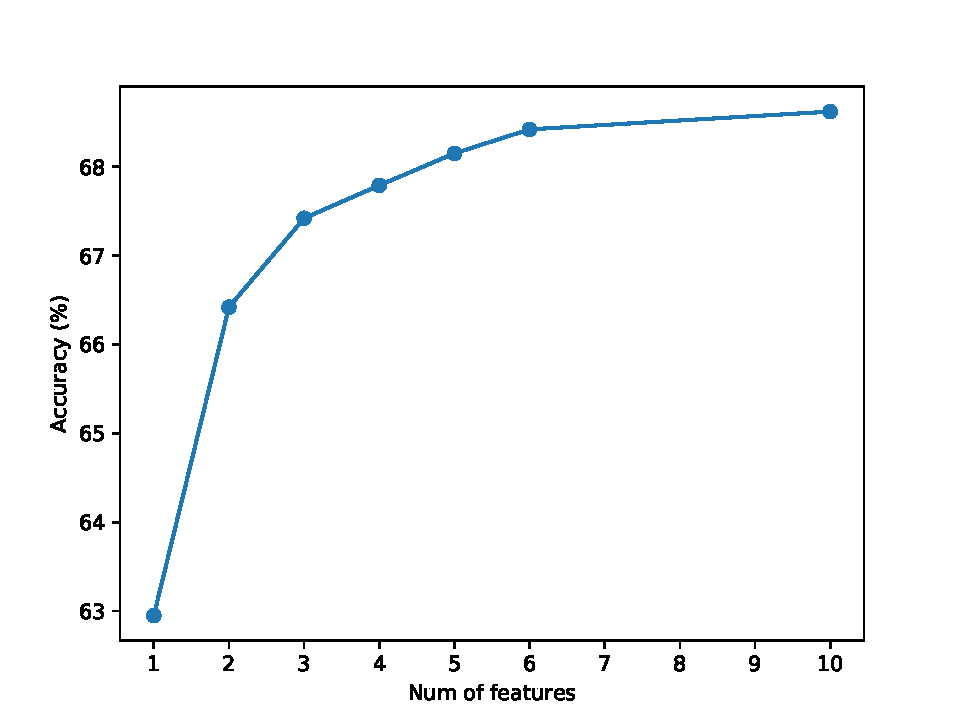
\includegraphics[width=0.8\textwidth]{feature_num.pdf}
  \caption{扩增倍数与网络精度关系曲线图}
  \label{fig:feature_num}
\end{figure}

\subsubsection{手工搜索实验与二值相似度分析}

在确定特征扩增倍数为2后,可以通过手工搜索的方式选择最优阈值。本文以0.05为间隔对基准网络的阈值设置进行了搜索。由于神经网络中激活值的均值一般在0附近,因此本文扩增倍数为2的两个阈值均设置为互为相反数。设置互为相反数的阈值既符合激活值的分布规律,也简化了搜索空间。不同固定阈值训练的第一阶段网络精度如表 \ref{tab:4} 所示,其中只标明了正数阈值,另一个阈值与其互为相反数。

\begin{table}[htb]
  \vspace{6pt}
  \centering
  \caption{不同固定阈值与网络精度的关系表}
  \label{tab:4}
  \begin{tabular}{cc}
    \toprule
    阈值取值   & Top-1精度(\%)    \\
    \midrule
    0.25 & 65.68 \\
    0.30 & 66.01 \\
    0.35 & 66.11 \\
    0.40 & 66.12 \\
    0.45 & 66.16 \\
    0.50 & 66.23 \\
    0.55 & 66.35 \\
    0.60 & 66.32 \\
    0.65 & 66.46 \\
    0.70 & 66.51 \\
    0.75 & 66.39 \\
    0.80 & 66.27 \\
    0.85 & 66.23 \\
    0.90 & 66.15 \\
    0.95 & 65.99 \\
    1.00 & 65.86 \\
    1.05 & 65.60 \\
    \bottomrule
  \end{tabular}
  \vspace{6pt}
\end{table}

可以看到,对相同网络设置不同阈值,ImageNet上的验证集精度可以相差1\%之多,本文的基准网络在使用-0.7和0.7作为阈值可以达到最好的效果,因此在后续实验中,所有与基准网络类似的网络在设置固定阈值时都使用-0.7和0.7。之前的研究\cite{unbalance}也指出阈值的设置对二值神经网络的性能会产生较大影响,但是没有解释阈值如何影响网络性能,在本文的多特征图方法中,可以用二值特征相似度解释不同阈值下网络精度的差异。不同阈值下网络精度和二值特征相似度的关系如图 \ref{fig:thres} 所示,本文ImageNet数据集中随机选择1000张图片作为输入,分别计算推理时的二值特征相似度,再将1000个二值特征相似度进行平均作为网络的二值特征相似度。不同阈值下,网络精度和二值特征相似度有明显相反的变化趋势,当二值特征相似度较低时,网络的精度较高。较低的二值特征相似度表示不同二值函数提取的二值特征差异性较大,从浮点特征保留的信息也更多,此时二值网络具有更强的特征表示能力。

\begin{figure}[htb]
  \centering
  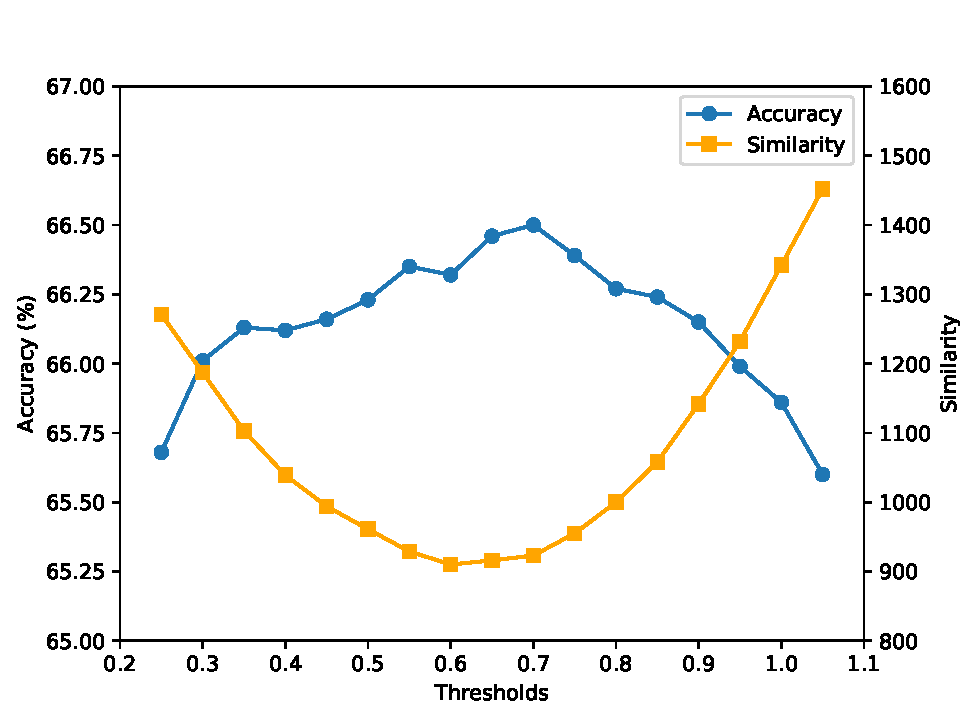
\includegraphics[width=0.8\textwidth]{thres.pdf}
  \caption{不同阈值下网络精度和二值特征相似度关系图}
  \label{fig:thres}
\end{figure}

\subsection{阈值迭代优化实验分析}

虽然手工搜索阈值可以得到相对较好的阈值取值,但是需要消耗大量的时间和资源,且不具有通用性。本文根据阈值参数的结构性特点,设计了阈值参数迭代优化算法,使阈值参数可以使用网络训练的方法自动寻优,简化了阈值选择的步骤。本文设计实验验证了阈值迭代优化方法的可行性。

本实验使用扩增倍数2和互为相反数的阈值,在网络中每层仅有一个阈值参数,另一个阈值直接取其相反数,训练时每层只对这一个阈值参数进行优化。本实验将对阈值的优化和对权重的优化拆分为两个步骤,步骤一中使用迭代优化算法对阈值进行优化,虽然这时也同时优化了权重,但不将该步优化的权重最为最终结果,步骤二中固定步骤一中得到的阈值,进行二值网络的两阶段训练,得到最终结果。为了节约时间,本实验仍然只训练两阶段中的第一阶段。不同初始阈值下迭代优化后训练网络第一阶段的精度和使用初始阈值作为固定阈值训练网络第一阶段的精度如表 \ref{tab:5} 所示。

\begin{table}[htb]
  \vspace{6pt}
  \centering
  \caption{不同初始阈值迭代优化方法与固定阈值方法精度对比表}
  \label{tab:5}
  \begin{tabular}{cccc}
    \toprule
    初始阈值   & \makecell{迭代优化步骤一\\Top-1精度(\%)} & \makecell{迭代优化步骤二\\Top-1精度(\%)} & \makecell{固定阈值\\Top-1精度(\%)}\\
    \midrule
    0.0 & 55.97 & 63.61 & 60.30 \\
    0.2 & 55.67 & 63.28 & 62.98 \\
    0.4 & 55.80 & 63.28 & 63.65 \\
    0.6 & 56.25 & 63.65 & 63.45 \\
    \bottomrule
  \end{tabular}
  \vspace{6pt}
\end{table}

可以看到,虽然固定阈值情况下不同初始阈值的网络训练精度相差较大,但是经过对阈值迭代优化后网络精度相差不大,在误差范围内。这表明阈值迭代优化算法对初始值的设置不敏感,无论如何设置初始值,都可以根据当前的二值网络结构自适应的将阈值优化到最优阈值附近。特别是初始值为0时同样可以优化到较好的效果,因此当使用新网络结构时,只需使用初始值为0的阈值进行迭代优化训练即可得到多特征图方法的合适阈值。

\subsection{多特征图方法有效性验证实验}

为了验证多二值特征图方法的信息保留能力,本文设计实验对比了有无多特征方法网络的推理精度。不调整网络通道数的情况下,使用扩增倍数为2的多特征图方法会使网络的整体计算量增加为原来的2倍。神经网络的基本规律表明,计算量的增加一般都会带来网络性能的提升,因此相同结构下使用多特征图方法的网络性能优于不使用多特征图方法的网络不能验证多特征图方法的有效性。为了在相同计算量的条件下进行比较多特征图方法的有效性,本文使用增加通道数的网络作为比较对象,扩增倍数为2的多特征图方法和增加通道数方法第一阶段网络训练精度如表 \ref{tab:6} 所示。

\begin{table}[htb]
  \vspace{6pt}
  \centering
  \caption{多特征图方法与增加通道数方法精度对比表}
  \label{tab:6}
  \begin{tabular}{ccccc}
    \toprule
    网络方法   & \makecell{首层卷积\\输出通道数} & OPs ($\times 10^8$) & Top-1精度(\%)& Top-1精度(\%) \\
    \midrule
    多特征图方法 & 32 & 0.84 & 70.15 & 89.29 \\
    增加通道数   & 45 & 0.89 & 69.15 & 88.53 \\
    增加通道数   & 64 & 1.61 & 70.05 & 89.00 \\
    \bottomrule
  \end{tabular}
  \vspace{6pt}
\end{table}

可以看到,在相同计算量的条件下多,特征图方法比增加通道数方法的Top-1精度高了1\%,这表明多特征图方法的浮点特征利用率更高。以网络中第二个卷积的输入特征图为例,相同网络整体计算量的条件下,多特征图方法的浮点特征有32通道,增加通道数的方法有45通道,但是多特征图方法的网络精度却更高,表明多特征图方法第二个卷积接收到的信息更多,更充分的利用了浮点特征。

与相近精度的增加通道数方法相比,多特征图方法节省了一般的计算量。同样网络中第二个卷积的输入特征图为例,性能接近的多特征图方法和增加通道数方法都提取到64通道的二值特征,说明二值网络的性能与二值特征承载的信息量有密切关系。但是多特征图方法却节省了大量的计算量,这表明二值特征的信息量并不于浮点特征的信息量成正比。事实上由于浮点特征的表示能力远大于二值特征,少量浮点特征的信息量需要大量二值特征才能充分表达。多二值特征图方法正是充分利用了浮点特征与二值特征不对称的信息量关系,以较少的计算量换取二值网络较大的性能提升。

\section{本章小结}

在本章中,本文针对二值神经网络特征表达能力不足的问题,提出了多二值特征图方法,实验表明该方法可以有效增加二值网络中的二值特征利用率。多二值特征图方法使用阈值可变的符号函数作为二值函数,通过设置不同的阈值设置不同的二值函数形式。为了衡量多二值特征保留浮点信息的能力,本文提出二值特征相似度的评价指标。阈值的设置是多二值特征图方法的核心,本文分析了阈值参数的基本性质,提出将阈值参数作为二值网络的结构参数看待,除了手工搜索阈值的方法外,本文还提出了迭代优化算法自适应学习阈值参数,实验验证迭代优化算法可以达到手工搜索得到的最优阈值的效果。
